\section{System}

%In this section, we first give an overview of our system
%for relation schema inferring,
%then we present the detail of each step in the system.
%%\KZ{Avoid the name RvSp, just say the system, or our system. Replace all
%%specific mentions of Freebase by more generic notion. This is possible
%%given that you have done the formal problem definition.}
%
%
%\subsection{System Overview}
% 3 main work: entity linking, relation merging, sel. pref.

\begin{figure*}[htp]
\centering \scalebox{0.65}{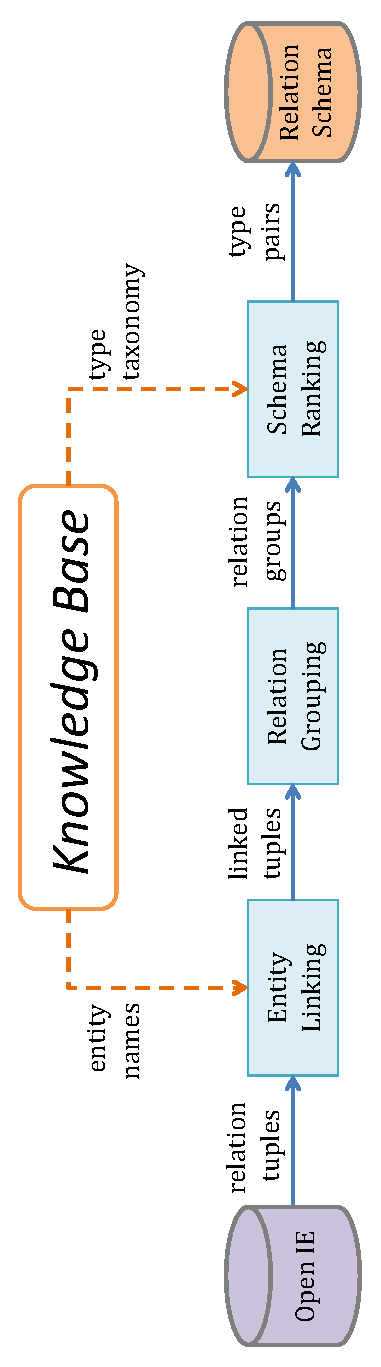
\includegraphics[angle=270]{system-crop.eps}}
%\epsfig{file=figure1-cropped.eps, width=2\columnwidth}
%\scalebox{0.35}
\caption{System Architecture}
\label{fig:workflow}
\end{figure*}
%\KZ{Redraw this figure as the three boxes in the middle turned out to be
%black in my version of PDF. Also, instead of naming ``ReVerb'' and ``Freebase''
%specifically, use generic terms like ``Open IE'' and ``Taxonomy''. We want
%this system to be general and not tied specifically to ReVerb or Freebase,
%though the actual implementation and eval are on ReVerb and Freebase. These
%we can say in the eval section.}

The workflow of our system is shown in Figure \figref{fig:workflow}.
% input: reverb relation, total 3 steps (2 sent)
The system takes Open IE relation tuples as the input,
then performs entity linking, relation grouping and schema ranking
to translate them into final ranked list of schemas.

% firstly, entity linking (3 sent)
{\bf(1) Entity Linking:}
Relation arguments are linked to entities in the knowledge base by
fuzzy string matching. Each entity in the knowledge base has a unique identifier.

% secondly, relation grouping (2 sent)
{\bf(2) Relation Grouping:}
Linked tuples sharing similar relation patterns are grouped together.
Besides, each group has a representative relation pattern, which is generated from all the patterns within the group.

% thirdly, simultaneously SP (3 sent)
% need to refine at the last sentence.
{\bf(3) Schema Ranking:}
For each linked tuple in one relation group, argument entities are transformed into types drawn from the knowledge base.
%The selectional association model considers both types simultaneously, and then produce a list of schemas for the relation group.
Then this procedure ranks type pairs (schemas) in terms of how much Open IE tuples a type pair can cover and how specific a type concept is.

\subsection{Entity Linking}

% 11 sentences

% main: tfidf for words on freebase
% based on overlap sim.
% pseudo code?
%


% 0. what are we going to do ?
% Given a relation tuple, we are going to find representative Freebase entities
% which stand for the arguments.
% 1. Formally definition
Formally, given $arg=(w_1,w_2,...,w_m)$, which contains $m$ words, we are going
to find a best Freebase entity standing for this argument, making relation tuples
to linked tuples, represented by $ltup=\langle ent1,\ rel,\ ent2 \rangle$.

% 2. ??? Talk about Freebase
% 3. each mid in FB has one or more entity names.
% example, China and PRC.
Each entity in Freebase has one or more aliases, forming $AList$. The default alias is the name of this entity.
For example, the entity \textit{m.02\_286} has the name ``New York City'' and other aliases
such as ``The Big Apple'' ``NYC'' and ``Empire City''.
% 4. leverage multiple namees to build an invert index.
We aim to support fuzzy matching between arguments and entity aliases,
so we take all the aliases into consideration, and build an inverted index
pointing words to all aliases that appear.

% 5. stop word set is used, and use the idf score to weight words.
Different words in one alias cannot be treated equally. Intuitively, a word
is more important if it occurs in fewer aliases, and vice versa.
Based on the inverted index, we use inverted document frequency score to
approximately model the weight of a word:
\begin{equation}
idf(w)=1\ /\ log(|\{alias : w \in alias\}|)
\end{equation}

\noindent
Besides, stop words are removed from aliases, treating their idf scores as 0.
% 6. matching rule: intersect >= N - 1, weighted overlap score >= threshold

In order to measure the probability of fuzzy matching from an argument to an alias,
we introduce the weighted overlap score:
\begin{equation}
overlap(arg, alias) = \frac {\sum\limits_{w \in arg \cap alias} idf(w)} {\sum\limits_{w \in arg \cup alias} idf(w)}
\end{equation}

\noindent
We merge all the aliases of an entity, producing the fuzzy matching score to entity level:
\begin{equation}
\begin{aligned}
score&(arg, ent) = \\
&\max\limits_{alias \in AList(ent)} overlap(arg, alias)
\end{aligned}
\end{equation}

For one argument having $n$ words (stop words are removed), we keep entities which has at least one alias
matching $n-1$ words in the argument, and has a matching score larger than a threshold, $\tau$.
% we can tune the threshold
% we can use formula to show the weighted score, that is intersect / union, weighed.
% 7. multiple matching, select the one with best wScore.
Once more than one entity is kept, we match the argument to the entity with highest matching score,
% 8. tie breaker: count occurrence in freebase relations.
if there still has a tie, the most popular entity is selected. The popularity of an entity is calculated
by counting number of relations it has in Freebase.
% 9. SUTime is used to map years and datetime.
In addition, we use SUTime \cite{chang2012sutime} to recognize dates, and directly
map these arguments to a pre-defined virtual entity (Freebase has \textit{type.datetime}
representing dates and times, but it doesn't contain any specified entities).
% check other papers, learn how to introduce FB without too much words.
% 10. discard non-match to guarantee accuracy of linking.
If one argument fails to link to any entity, the corresponding relation tuple is discarded.
% Ranking Method May Change?
%   use wScore threshold to filter entities
%   then sorting by interLen, then popularity ??? (maybe we can have a try afterwards)
%


%\begin{table}[htbp]
%	\centering
%	\caption{Syntactic Transform Rules}
%	\begin{tabular}{|l|l|}
%		%\toprule
%        \whline
%		Category & Pattern Template \\
%		%\midrule
%        \hline
%        % Continuous Tense & \{$adv_1$\} \textbf{be} \{$adv_2$\} verb:VBG \{text\}
%        %                  & $verb_{lem}$ \{phrase\} \\
%		% Participle Tense & \{$adv_1$\} \textbf{have} \{$adv_2$\} verb:VBN \{text\}
%        %                  & $verb_{lem}$ \{phrase\} \\
%        % Participle + Passive & \{$adv_1$\} \textbf{have} \{$adv_2$\} been \{text\}
%        %                      & is \{text\} \\
%        Continuous Tense & \textbf{be} verb:VBG \{phrase\} \\
%		Participle Tense & \textbf{have} verb:VBN \{text\} \\
%        Future Tense & \textbf{will}/\textbf{shall} verb:VB \{pharse\} \\
%                     & \textbf{be} going to verb:VB \{phrase\} \\
%		%\bottomrule
%        \whline
%	\end{tabular}%
%	\label{tab:synt rules}%
%\end{table}


\subsection{Relation Grouping}
% 8 sents.
% 1. group tuples together, give definition
%A relation group consists of linked tuples sharing similar relation patterns,
%along with a representative pattern.
% 2. same & syntactically similar rel. patterns will be in a group, no overlapping.
%Each linked tuple belongs to one unique group.
In the step of relation grouping, linked tuples with similar relation patterns form a group.
Each linked tuple belongs to one unique group.

% 1. what is similar ?

% 3. algorithm: syntactic rules to convert tense,
% mainly focus on 3 tense: will/should/must be, be -ing, participle

%We define syntactically equivalence between two relation patterns, as both of them can be converted
%into the same simple pattern by a list of transformations.
%Every relation pattern in one group is equivalent with each other.
The idea is to simplify relation patterns by syntactic transformations.
If two patterns share the same simplified pattern, we treat them as
being equivalent and put them into one group.
First, since adjectives, adverbs and modal verbs can hardly change the
type distribution of arguments in a relation,
we remove these words from a pattern.
Second, many relations from Open IE contain verbs, which come in
different tenses. We transform all tenses into present tense.
In addition, passive voice in a pattern, if any, is kept in
the transformed pattern.
% 4. Create a table, showing the rules to find them.
%The detail of syntactic rules is shown in Table 1.
%\KQ{refer to Liang et al., 2014 to build the rule table, containing continuous, participle, be-the-name-of
%and passive form}
% For example, a --> b
% check liang's 14 paper to learn the representation of tables.
% 5. use stanford parser to tokenize & postag.
% 6. representative relation: present tense
A simple example below shows a group of relations:
\begin{center}
    $\langle$X, \textit{resign from}, Y$\rangle$
    
    $\langle$X, \textit{had resigned from}, Y$\rangle$
    
    $\langle$X, \textit{finally resigned from}, Y$\rangle$
\end{center}

All linked tuples with the same simplified pattern form a group.
This pattern is selected as the representative pattern, like the pattern \textit{``resign from''}
in the above example.


\subsection{Ranking}
\label{sec:ranking}

%The ranking phase takes the soft clustering results from the previous phase 
%and ranks both the clusters and the words in each cluster.

% Note that the clusters of words from previous phase are not ordered. 
% But in practical product reviewing, the aspects should be treated differently. 
% As mentioned in \secref{sec:intro}, the ranking of the aspects should 
% reflect the opinion of the users. 
% \KZ{I don't quite understand this...
% Do you mean that if users pay more attention to one aspect, this aspect should
% be ranked higher? The above needs to be rephrased.} 
% Also the quality of the clusters, i.e.,
% how related are the words to the aspect - may vary, due to different frequencies of the aspects in the corpus. \KZ{Don't understand the above either. I assume
% you want to return the top relevant words to an aspect cluster as the most
% representative aspect word. But why is it related to the frequency of the 
% aspect in the corpus?}
% Also, as mentioned in 
% \secref{sec:system_overview}, the clustering is mainly based on 
% co-occurrence of words, which may not fully capture the semantic 
% relatedness of words. \KZ{Why not?} Motivated by these, 
% we proposed to do a 2-stage ranking based on the clustering result, 
% with the help of knowledge bases: first rank the aspect clusters, 
% then the words in each cluster.

Some aspect clusters extracted from hotel reviews are shown in \tabref{table:cluster_example}.
Each row is an aspect cluster with words ranked by word distribution.
We manually select the best aspect words for each cluster and show them in boldface.
These aspect words act as representatives of other words in the corresponding cluster,
 so they should be at the center of the clusters semantically.
However, it can be seen that not all chosen words have the highest frequency.
In order to not only provide such aspect clusters, 
but also automatically select the best aspect words,
in the following ranking phase we adjust the word rankings by taking the semantic
distance between words into consideration.

\begin{table}[t]
\centering
\begin{tabular}{|l|} \hline
breakfast, meal, \textbf{food}, tasty, dinner, ... \\\hline
\textbf{staff}, desk, service, friendly, reception, ... \\\hline
close, city, \textbf{location}, place, central, ... \\\hline
bed, shower, spacious, \textbf{room}, size, ... \\\hline
\hline
\end{tabular}
\caption{Several aspect clusters extracted from hotel reviews.
  Each row shows the candidate words of an aspect, sorted by the weight of each word. 
Bold-faced words are the chosen representatives of each aspect cluster.}
\label{table:cluster_example}
\end{table}

When ranking words in each cluster, we want to make sure that one word doesn't appear at top in multiple clusters. We first calculate a confidence score of each cluster based on their distinctiveness: if the word distribution of one cluster is different from all other clusters, it has a high confidence score and we process it first. When ranking the words within each cluster, we also consider the clusters that have already been ranked, that is, clusters with higher confidence scores.

\subsubsection{Ranking Clusters}
\label{sec:ranking_clusters}

As analyzed in the previous section, the noise in each cluster is introduced by the overlap between clusters. We follow this direction and propose a measurement for the quality of clusters based on their distinctiveness.
The \textbf{distinctiveness} of a cluster measures how 
different is its word distribution from other clusters'. 
Intuitively, a cluster is of high quality when it has small overlapping 
with other clusters. We measure this by calculating the weighted sum of 
mutual information of the words within the cluster against all other clusters. 

The mutual information of two random variables is a measure for the mutual dependence. For random variables $X$ and $Y$, their mutual information is defined by 
\begin{equation}
MI(X, Y) = \sum_{y\in Y} \sum_{x\in X} p(x, y) \log\left(\frac{p(x, y)}{p(x)p(y)}\right) \label{eq:mi}
\end{equation}

Let $a$ be a word in cluster $c, c\in[1,C]$ with frequency $f(c, a)$. 
Let $S(c, a)$ be the score of word $a$ in cluster $c$, 
then the score of the cluster $c$, $S(c) = \sum_{a} S(c, a)$. 
$S(c,a)$ is calculated by the mutual information between $a$'s appearance 
in cluster $c$ and $a$ in all other clusters. 

\begin{align*}
	S(c, a) &= \log\left(\frac{f_c(a)}{\sum_{r\in[1, C], r\neq c} f_r(a)}\right) \\
			&= \log(f_c(a)) - \log(\sum_{r\in[1, C], r\neq c} f_r(a))
    S(c) &= \sum_{a} S(c, a) \\
         &= \sum_{a} \sum_{d\in [1, C], d\neq c} MI(a_c, a_d) \\
         &= \sum_{a} \sum_{d\in [1, C], d\neq c} 
\end{align*}

Finally the clusters are ranked in decending order of the score. 

\subsubsection{Ranking Words}
\label{section:ranking_words}

Each cluster consists of words related to a potential aspect and we want 
to find what is the aspect. We do this by finding the word that best 
summarizes each cluster. For ranking the words in one cluster on how they 
summarize the cluster, we leverage the intuition behind Lesk 
lemmatization algorithm and WordNet to 
define a \emph{semantic similarity} $\sims(w_1, w_2)$ between words $w_1$ and $w_2$.
The semantic similarity measures how much the two words are related. 
The similarity consists of two parts:

\begin{itemize}
    \item Path similarty $\sims_p$ is calculated by the shortest path that connects two words in the is-a (hypernym/hyponym) taxonomy. The scores range from 0 to 1. \KZ{This is a very old and rudimentary use of WordNet. However, it doesn't
work very well because the distance between any pair of hypernym/hyponym is
actually different.}
    \item Definition overlap $\sims_d$ is calculated based on 
the gloss paragraphs of the two words in WordNet. \KZ{Elaborate further as
this step seems crucial?}
We train a recurrent neural network language model on a large dataset 
and use it to embed the paragraphs, then calculate the cosine of the two embedding vectors as the similarity of of the two definitions.
\end{itemize}

The final semantic similarity score is calculated by $\sims(w_1, w_2) = \sims_p(w_1, w_2) + \sims_d(w_1, w_2)$. When ranking words inside each cluster, we start with the clusters with high confidence, by the order calculated from the previous step. For word $w$ in cluster $i$, there is a weight, $u_{w,i}$, assigned by the LDA. When calculating the score of word $w$ in cluster $i$, denoted by $s_{w,i}$, we also consider its score from all previous clusters $1\sim i-1$, $s_{w,1} \sim {w,i-1}$. Similar to cluster ranking, we consider the mutual information, resulting in the final calculation of the score:
$$s_{w,i} = u_{w,i} \sum_{w'} \sims(w, w') - \sum_{j=1}^{i-1} s_{w,j}$$
\KZ{What's the intuition for doing the above? What if you don't do it just just
treat each cluster independently? Can we have some evaluation results on this?
Generally in this method section, there are many design decision made. We
need to justify them carefully either by intuition, or by citation (previous
work) and it would be the best if we can substantiate them using eval results.}

The final word order in each cluster is sorted by this score.

